% ============================================================
%  第五章 电子-声子相互作用（§1–§5 + 章末参考文献）
%  底本：高等教育出版社《固体理论》（第二版）印刷页 138–158
%  （PDF 页 = 印刷页 + 20，章名页 PDF p158，末页 PDF p178）
%  OCR 输入：MinerU/full_merged.md 行 6404–7197
%  公式编号自检：§1 (5.1.1)–(5.1.4)；§2 (5.2.1)–(5.2.31)；
%    §3 (5.3.1)–(5.3.20)；§4 (5.4.1)–(5.4.22)；§5 (5.5.1)–(5.5.20)。
%    共 97 个编号，全部自动编号，逐一对上原书。
%  缺号判定（对照原书页面）：任务单所示 3 处缺号均为 OCR 漏检而非原书跳号——
%    (5.2.16)：OCR 残 tag {2.16}，原书 p142 有此式，已补全；
%    (5.2.31)：N 过程跃迁概率大式 OCR 无 tag，原书 p145 有编号，已补排；
%    (5.4.10)：H_ep 一般式 OCR 乱码无 tag，原书 p149 有编号，已按原书重排；
%    (5.5.3) ：有效互作用矩阵元式 OCR 无 tag，原书 p154 有编号，已补排。
%    故本章实有编号公式 97 个（OCR tag 计数 94 ＋ 补排 3）。
%  已修正的 OCR/原书错误：
%  1. (5.1.4) 被拆成相邻两个 $$ 块（首行无号＋次行带号），按原书 p139
%     合并为一个编号公式
%  2. §1 "其中ε.是带边能量…"段 ε_c 重复串入、式(5.1.2)后杂符 $\pmb{c}_1$ 等，
%     按 p138 复原为"其中 ε_c 是……通常称为形变势，而 c_1 相应地称为……
%     式(5.1.2)就是电子-声子互作用的形变势模型[1]…"
%  3. (5.2.3) 第三行 V(r_i−l) 原书排印如此，按求和指标 j 与 ≡Σ_j h(r_j)
%     更正为 V(r_j−l)（原书排印错误）
%  4. (5.2.8) 第二行求和 Σ_{k,ν}→Σ_{k,k'}（OCR 误识，p141）
%  5. (5.2.10) (a_qs+q⁺_{−qs}) 原书排印如此，按 (5.2.9) 更正为
%     (a_qs+a⁺_{−qs})（原书排印错误）
%  6. (5.2.14) 末尾因子 e^{i(k−k')·l} OCR 漏失，按 p162 补
%  7. (5.2.16) OCR tag 残缺为 {2.16}、求和下标乱码（∑_{p'}、"(5.2.5),"串入），
%     按 p142 重排补全
%  8. §2 "分别代 e_qs 表 LA 与 TA 声子"→"分别代表 LA 与 TA 声子"（p143，
%     OCR 串入公式）；(ii) 段 X_n、k_n→K_n（OCR 误识＋原书小写排印）
%  9. §2 "总动量守恒条件相差hK，……所造 ħK_n 成的"按 p144 复原为
%     "相差 ħK_n，……所造成的"；"满足 j⃗格的动量守恒条件"按 p144 为
%     "满足严格的动量守恒条件"；"正格矢 a_i 0"补箭头 a_i→0
% 10. (5.2.27) 第二行箭头及条件 OCR 乱码，按 p145 为"(t 大时)⟹"；
%     (5.2.29) 的 S→δ；(5.2.28) ħω_{±q} 按原书
% 11. (5.2.31)：N 过程跃迁概率大式 OCR 无 tag 且排乱，原书 p145 有编号
%     (5.2.31)，已按原书重排补入；其下"(已占据态)(空占态)"处的 (n_k=1)
%     按 p145 补
% 12. §3 "这里晶体取单体积"→"单位体积"（p146）；(5.3.6)(5.3.7) 的 \frac{}{}
%     残缺按 p147 复原；(5.3.14) 相邻两块按原书（p147–148 跨页一式）合并；
%     (5.3.17) 整式 \textsf 乱码按 p148 重排
% 13. §4 (5.4.1) 首行 OCR 漏 e_q，按 p148 补为 e_q Q_q；(5.4.3) \sqrt{ΛM}→
%     \sqrt{NM}，W(r)=√(NM){u₊−u₋} 按 p149 复原
% 14. (5.4.10)：H_ep 一般式 OCR 严重乱码无 tag，原书 p149 有编号 (5.4.10)，
%     已按原书重排补入（C⁺_{k'} 的 k' 按 300dpi 页面核实）
% 15. §4 "−eφ(r) 代表处电子受 LO 声子…"按 p149 补"r"→"代表 r 处电子"；
%     "随 g 增大"→"随 q 增大"；"L0 声子"→"LO 声子"；"声子能量 hω1"→ħω_L；
%     OCR 串入的 ħω_L、Δt、α、q 等杂符已删（p151–152）
% 16. (5.4.19) 首行关系号按 p151 为 "≡"（OCR 作 =）
% 17. <N_ph>：OCR 乱码（\vec p\vec circ），按 p151 为 <N_声>（汉字下标"声"）
% 18. §4 "只有少数 Ⅱ-Ⅴ 族"按 p152 为"Ⅲ-Ⅴ族和 Ⅱ-Ⅵ族化合物半导体"；
%     表 5.1 的 MδgO→MgO、zns→ZnS、"5 InSb"→InSb
% 19. (5.5.2) 第二项分母 (ε_k−ε_{k+q}−ħω_{−q}) OCR 漏失，按 p153 补
% 20. (5.5.3)：有效互作用矩阵元式 OCR 无 tag，原书 p154 有编号 (5.5.3)，
%     已补排
% 21. §5 "|m_1|与图 5.7 中(a)对应"→|m_1⟩（OCR 键错）；"其中|n>Z|m>为 H_0
%     的本征态"→"|n>及|m>"（p156）
% 22. (5.5.16) 相邻两块按原书（p156–157 跨页一式）合并为一个编号公式；
%     (5.5.18) 分子 C_{kq}→C_{kσ}（p157）
% 23. §5 末段 "|ε_k−ε_{k+q}|<ħω_k" 原书排印如此，按同段能壳区条件更正为
%     ħω_q（原书排印错误）；ε_{k+q}、ω_q、ħω≡|ε_k−ε_{k+q}| 等乱码按
%     p157–158 复原；"由于晶格畸变以ω。频率响应电子(1)"→ω_q（OCR）
% 24. 文献[4][5] "Frohlich"按 p158 原书为"Fröhlich"，[4] 有 et al.
% 25. 其余：全角句点"．"→ASCII "."；OCR 间隔符 ~ 删除；\mathrm{d} 收紧；
%     \hat{δ}/\widehat{δ}→δ；\varrho→ρ；\epsilon 与 \varepsilon 统一为
%     \varepsilon；被拆散的"玻$n_q$色""决 定"等按原书合并
%  遗留问题：
%  · §1 "类似的，a_qC⁺_{k−q}C_k 也可以代表吸收声子后产生电子-空穴对"一句
%    原书即印作 C⁺_{k−q}（而图 5.2(b) 为 C⁺_{k+q}），两处照原书照录未改；
%  · §2 "将写出自旋为下一章讨论超导用"原书如此（无逗号），照录；
%  · 图 5.1–5.7 均为占位图（fig5-N.pdf），宽度按原书目测配置。
% ============================================================
\chapter{电子-声子相互作用}

\section{互作用过程}

能带论只计及了晶格周期势场对电子的作用.当考虑晶格振动时，由于原子（离子）偏离平衡位置会破坏周期场，引起势能的改变，将使能带电子受到晶格位移所产生附加势场的作用，这就是电子和晶格振动的相互作用.晶格振动由声子描述，因此这个互作用又称为电子与声子的相互作用.

在能带极值附近，波矢 $\boldsymbol{k}$ 和有效质量 $m$ 的电子能量可近似写为
\begin{equation}
  \varepsilon_k=\varepsilon_{\mathrm{c}}+\frac{\hbar^2k^2}{2m}
\end{equation}
其中 $\varepsilon_{\mathrm{c}}$ 是带边能量，可理解为能带电子的势能.如果不考虑晶格振动，则 $\varepsilon_{\mathrm{c}}$ 代表晶格周期势对电子的作用，它随晶格常数变化.由于格波的纵声学模（LA 声子）总是伴随着晶体体积和晶格常数的局域变化，因此存在晶格振动时，带边能量将发生移动
\begin{equation}
  \delta\varepsilon_{\mathrm{c}}=\left(\frac{\partial\varepsilon_{\mathrm{c}}}{\partial V}\right)\delta V
  =V\left(\frac{\partial\varepsilon_{\mathrm{c}}}{\partial V}\right)\left(\frac{\delta V}{V}\right)
  =c_1\Delta\left(\boldsymbol{r}\right)
\end{equation}
其中 $\Delta\left(\boldsymbol{r}\right)$ 是体积的相对变化，它反映晶格局域形变的大小，称为形变量.因此 $\delta\varepsilon_{\mathrm{c}}$ 代表晶格振动的形变所引起单电子势能的变化，通常称为形变势，而 $c_1$ 相应地称为形变势常数，其数值由实验确定.式(5.1.2)就是电子-声子互作用的形变势模型\textsuperscript{[1]}，广泛应用于金属和半导体问题.

在长波近似下，根据式(2.5.31)，可以用 LA 声子的产生算符 $a_q^{+}$ 与消灭算符 $a_q$ 表示 $\Delta\left(\boldsymbol{r}\right)$，即
\begin{equation}
  \Delta\left(\boldsymbol{r}\right)=\nabla\cdot\boldsymbol{u}\left(\boldsymbol{r}\right)
  =\mathrm{i}\sum_{q}\sqrt{\frac{\hbar}{2\rho V\omega_q}}
  \left(\boldsymbol{e}_q\cdot\boldsymbol{q}\right)
  \left(a_q\mathrm{e}^{\mathrm{i}\boldsymbol{q}\cdot\boldsymbol{r}}
  -a_q^{+}\mathrm{e}^{-\mathrm{i}\boldsymbol{q}\cdot\boldsymbol{r}}\right)
\end{equation}
电子-声子互作用的二次量子化表示式由单体势 $\delta\varepsilon_{\mathrm{c}}$ 对态向量的平均决定，即
\begin{equation}
\begin{aligned}
  H_{\mathrm{ep}}&=\int\mathrm{d}\boldsymbol{r}\,\varPsi^{+}\left(\boldsymbol{r}\right)
  c_1\Delta\left(\boldsymbol{r}\right)\varPsi\left(\boldsymbol{r}\right)\\
  &=\mathrm{i}c_1\sum_{k,q}\sqrt{\frac{\hbar}{2\rho V\omega_q}}
  \left(\boldsymbol{e}_q\cdot\boldsymbol{q}\right)
  \left(a_qC_{k+q}^{+}C_k-a_q^{+}C_{k-q}^{+}C_k\right)
\end{aligned}
\end{equation}
式(5.1.4)给出电子-声子互作用的两个基本过程：(a)$\boldsymbol{k}$ 电子吸收 $\boldsymbol{q}$ 声子变为 $\boldsymbol{k}+\boldsymbol{q}$ 态上的电子；(b)$\boldsymbol{k}$ 电子发射 $\boldsymbol{q}$ 声子变为 $\boldsymbol{k}-\boldsymbol{q}$ 态上的电子.用二次量子化术语说：$a_qC_{k+q}^{+}C_k$ 为消灭 $\boldsymbol{k}$ 电子和 $\boldsymbol{q}$ 声子并产生 $\boldsymbol{k}+\boldsymbol{q}$ 电子，如图5.1(a)所示.$a_q^{+}C_{k-q}^{+}C_k$ 则代表 $\boldsymbol{k}$ 电子被消灭和 $\boldsymbol{q}$ 声子与 $\boldsymbol{k}-\boldsymbol{q}$ 电子产生，由图5.1(b)表示.

\begin{center}
\begin{minipage}{7.5cm}
\centering
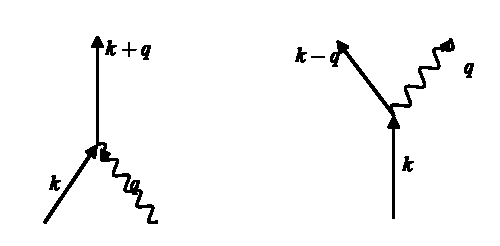
\includegraphics[width=7.5cm]{fig5-1.pdf}\\[0.3em]
{\small (a) $a_qC_{k+q}^{+}C_k$ 声子吸收\qquad\qquad (b) $a_q^{+}C_{k-q}^{+}C_k$ 声子发射}\\[0.2em]
{\small 图 5.1\quad 电子-声子互作用的一级过程}
\end{minipage}
\end{center}

当 $\boldsymbol{k}$ 在费密球外而 $\boldsymbol{k}-\boldsymbol{q}$ 在费密球内时，$a_q^{+}C_{k-q}^{+}C_k$ 将代表消灭 $\boldsymbol{k}$ 电子和 $\boldsymbol{k}-\boldsymbol{q}$ 空穴，并产生 $\boldsymbol{q}$ 声子，即常见的电子-空穴对复合发射声子的过程.类似的，$a_qC_{k-q}^{+}C_k$ 也可以代表吸收声子后产生电子-空穴对.在图5.2中箭头朝上代表电子，箭头朝下代表空穴.

\begin{center}
\begin{minipage}{8cm}
\centering
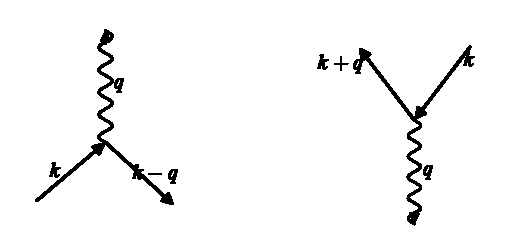
\includegraphics[width=8cm]{fig5-2.pdf}\\[0.3em]
{\small (a) $a_q^{+}C_{k-q}^{+}C_k$ 电子-空穴对复合发射声子\qquad (b) $a_qC_{k+q}^{+}C_k$ 吸收声子产生电子-空穴对}\\[0.2em]
{\small 图 5.2\quad 电子-空穴对的产生与复合}
\end{minipage}
\end{center}

以上是 $H_{\mathrm{ep}}$ 的一级微扰过程，它用于解释晶体的输运特性，如电阻的成因等.电子-声子互作用的高阶微扰过程由上述基本过程组成，例如二级微扰的下列3个图形［图5.3(a)、(b)、(c)］.图形(a)为电子在运动时先发射后吸收 $\boldsymbol{q}$ 声子，物理实质是电子带着晶格畸变运动，这必然会对电子自身的能量产生修正，称为电子自能修正图.图形(b)代表声子自能修正，因为电子系统对声子扰动场的屏蔽，将改变离子间的互作用势，从而对声子频率产生修正.图形(c)则是两个电子通过声子的间接互作用，在一定条件下将成为电子之间的有效吸引势，它是产生超导电性的主要机制.在§3—§5中我们将结合具体问题讨论这3个二级过程.

\begin{center}
\begin{minipage}{10.5cm}
\centering
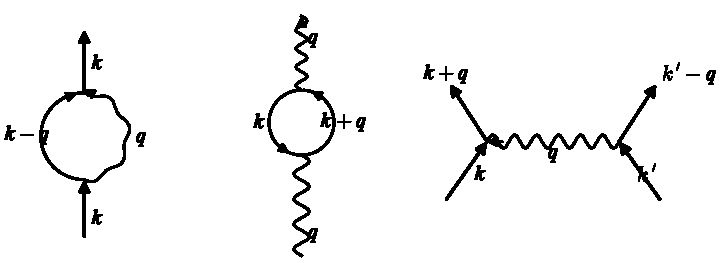
\includegraphics[width=10.5cm]{fig5-3.pdf}\\[0.3em]
{\small (a) 电子自能修正\qquad (b) 声子自能修正\qquad (c) 电子-声子-电子互作用}\\[0.2em]
{\small 图 5.3\quad 二级过程}
\end{minipage}
\end{center}

\section{电子与声频支声子的相互作用}

以上是电子与声子互作用的连续模型，而更严格的推导应当从晶格模型出发\textsuperscript{[2]}.对于简单晶格只有声频支振动，电子与晶格振动的相互作用就是电子与声频声子的互作用.设 $\boldsymbol{l}$ 格点上离子与 $j$ 电子（位置由 $\boldsymbol{r}_j$ 表示）之间的相互作用势能为 $V\left(\boldsymbol{r}_j-\boldsymbol{l}\right)$，则当离子不动时电子与离子的互作用为
\begin{equation}
  H_{\mathrm{ei}}^{0}=\sum_{j,l}V\left(\boldsymbol{r}_j-\boldsymbol{l}\right)
\end{equation}
它表示电子在周期场中的势能，这里 $\boldsymbol{l}\equiv\boldsymbol{R}_l=\sum_{i}l_i\boldsymbol{a}_i$.实际上离子在不断地振动，其相对位移为 $\boldsymbol{u}_l\left(t\right)$，电子与离子互作用应当是
\begin{equation}
  H_{\mathrm{ei}}=\sum_{j,l}V\left(\boldsymbol{r}_j-\boldsymbol{l}-\boldsymbol{u}_l\right)
\end{equation}
因此，能带电子与晶格振动的相互作用由式(5.2.2)与式(5.2.1)之差表示
\begin{equation}
\begin{aligned}
  H_{\mathrm{ep}}&=H_{\mathrm{ei}}-H_{\mathrm{ei}}^{0}\\
  &=\sum_{j,l}\left\{V\left(\boldsymbol{r}_j-\boldsymbol{l}-\boldsymbol{u}_l\right)
  -V\left(\boldsymbol{r}_j-\boldsymbol{l}\right)\right\}\\
  &=-\sum_{j,l}\boldsymbol{u}_l\cdot\nabla V\left(\boldsymbol{r}_j-\boldsymbol{l}\right)
  \equiv\sum_{j}h\left(\boldsymbol{r}_j\right)
\end{aligned}
\end{equation}
其中电子与声子互作用的单体势为
\begin{equation}
  h\left(\boldsymbol{r}\right)=-\sum_{l}\boldsymbol{u}_l\cdot\nabla V\left(\boldsymbol{r}-\boldsymbol{l}\right)
\end{equation}
若选布洛赫函数
\begin{equation}
  \psi_k\left(\boldsymbol{r}\right)=u_k\left(\boldsymbol{r}\right)\mathrm{e}^{\mathrm{i}\boldsymbol{k}\cdot\boldsymbol{r}}
  \text{，}\quad u_k\left(\boldsymbol{r}+\boldsymbol{l}\right)=u_k\left(\boldsymbol{r}\right)
\end{equation}
作为电子系统二次量子化态向量的基函数，则
\begin{equation}
  \varPsi\left(\boldsymbol{r}\right)=\sum_{k}C_k\psi_k\left(\boldsymbol{r}\right)
  \text{，}\quad \varPsi^{+}\left(\boldsymbol{r}\right)=\sum_{k}C_k^{+}\psi_k^{+}\left(\boldsymbol{r}\right)
\end{equation}
式中 $C_k^{+}$ 和 $C_k$ 为能带电子的产生及消灭算符，满足费密子的反对易关系
\begin{equation}
  \left[\,C_k,C_{k'}^{+}\,\right]_{+}=\delta_{kk'}\text{，}
  \left[\,C_k,C_{k'}\,\right]_{+}=\left[\,C_k^{+},C_{k'}^{+}\,\right]_{+}=0
\end{equation}
为了记号简单起见在这里暂不标明自旋指标 $\sigma$，只需注意对 $\boldsymbol{k}$ 求和应包括自旋简并度.在§5中讨论电子间有效吸引互作用时，将写出自旋为下一章讨论超导用.

从单体势容易求出用电子算符表示的电子-声子互作用为：
\begin{equation}
\begin{aligned}
  H_{\mathrm{ep}}&=\int\varPsi^{+}\left(\boldsymbol{r}\right)h\left(\boldsymbol{r}\right)\varPsi\left(\boldsymbol{r}\right)\mathrm{d}\boldsymbol{r}\\
  &=\sum_{k,k'}\left\langle k'\left|h\left(\boldsymbol{r}\right)\right|k\right\rangle C_{k'}^{+}C_k\\
  &=-\sum_{l}\sum_{k,k'}\boldsymbol{u}_l\cdot\left\langle k'\left|\nabla V\left(\boldsymbol{r}-\boldsymbol{l}\right)\right|k\right\rangle C_{k'}^{+}C_k
\end{aligned}
\end{equation}
再将晶格振动用声子算符表示
\begin{equation}
  \left.\begin{aligned}
  \boldsymbol{u}_l&=\frac{1}{\sqrt{NM}}\sum_{q,s}\boldsymbol{e}_{qs}Q_{qs}\mathrm{e}^{\mathrm{i}\boldsymbol{q}\cdot\boldsymbol{l}}\\
  Q_{qs}&=\sqrt{\frac{\hbar}{2\omega_{qs}}}\left(a_{qs}+a_{-qs}^{+}\right)\\
  \boldsymbol{e}_{qs}&=\boldsymbol{e}_{-qs}\text{，}\ \left|\boldsymbol{e}_{qs}\right|=1
  \end{aligned}\right\}
\end{equation}
代入式(5.2.8)，求得 $H_{\mathrm{ep}}$ 的二次量子化表示
\begin{equation}
\begin{aligned}
  H_{\mathrm{ep}}&=-\sum_{l}\sum_{k,k'}\sum_{q,s}\left(\frac{\hbar}{2NM\omega_{qs}}\right)^{1/2}
  \left(a_{qs}+a_{-qs}^{+}\right)C_{k'}^{+}C_k\mathrm{e}^{\mathrm{i}\boldsymbol{q}\cdot\boldsymbol{l}}\times\\
  &\quad\left\{\boldsymbol{e}_{qs}\cdot\left\langle k'\left|\nabla V\left(\boldsymbol{r}-\boldsymbol{l}\right)\right|k\right\rangle\right\}
\end{aligned}
\end{equation}
其中 $N$ 为元胞数，$M$ 为离子质量，$s$ 代表格波的偏振指标.布洛赫函数的积分
\begin{equation}
  \left\langle k'\left|\nabla V\left(\boldsymbol{r}-\boldsymbol{l}\right)\right|k\right\rangle
  =\int\mathrm{d}\boldsymbol{r}\,u_{k'}^{*}\left(\boldsymbol{r}\right)u_k\left(\boldsymbol{r}\right)
  \mathrm{e}^{\mathrm{i}\left(\boldsymbol{k}-\boldsymbol{k}'\right)\cdot\boldsymbol{r}}\nabla V\left(\boldsymbol{r}-\boldsymbol{l}\right)
\end{equation}
由于晶体满足周期性边界条件，作 $\boldsymbol{r}\to\boldsymbol{r}+\boldsymbol{l}$ 代换积分不变，再利用 $\boldsymbol{u}_k\left(\boldsymbol{r}+\boldsymbol{l}\right)=\boldsymbol{u}_k\left(\boldsymbol{r}\right)$，可将上式简化为
\begin{equation}
\begin{aligned}
  &\left\langle k'\left|\nabla V\left(\boldsymbol{r}-\boldsymbol{l}\right)\right|k\right\rangle\\
  &=\left\{\int\mathrm{d}\boldsymbol{r}\,u_{k'}^{*}\left(\boldsymbol{r}\right)u_k\left(\boldsymbol{r}\right)
  \mathrm{e}^{\mathrm{i}\left(\boldsymbol{k}-\boldsymbol{k}'\right)\cdot\boldsymbol{r}}\nabla V\left(\boldsymbol{r}\right)\right\}
  \mathrm{e}^{\mathrm{i}\left(\boldsymbol{k}-\boldsymbol{k}'\right)\cdot\boldsymbol{l}}
\end{aligned}
\end{equation}
对离子势作傅里叶展开
\begin{equation}
  V\left(\boldsymbol{r}\right)=\sum_{p}V_p\mathrm{e}^{\mathrm{i}\boldsymbol{p}\cdot\boldsymbol{r}}
\end{equation}
可求得
\begin{equation}
  \left\langle k'\left|\nabla V\left(\boldsymbol{r}-\boldsymbol{l}\right)\right|k\right\rangle
  =\mathrm{i}\sum_{p}\boldsymbol{p}V_p\left\langle k'\left|\mathrm{e}^{\mathrm{i}\boldsymbol{p}\cdot\boldsymbol{r}}\right|k\right\rangle
  \mathrm{e}^{\mathrm{i}\left(\boldsymbol{k}-\boldsymbol{k}'\right)\cdot\boldsymbol{l}}
\end{equation}
其中
\begin{equation}
  \left\langle k'\left|\mathrm{e}^{\mathrm{i}\boldsymbol{p}\cdot\boldsymbol{r}}\right|k\right\rangle
  =\int\mathrm{d}\boldsymbol{r}\,u_{k'}^{*}\left(\boldsymbol{r}\right)u_k\left(\boldsymbol{r}\right)
  \mathrm{e}^{\mathrm{i}\left(\boldsymbol{k}+\boldsymbol{p}-\boldsymbol{k}'\right)\cdot\boldsymbol{r}}
\end{equation}
将式(5.2.14)代入式(5.2.10)
\begin{equation}
\begin{aligned}
  H_{\mathrm{ep}}&=-\mathrm{i}\sum_{k,k'}\sum_{q,s}\sum_{p}\left(\frac{N\hbar}{2M\omega_{qs}}\right)^{1/2}
  \left(\boldsymbol{e}_{qs}\cdot\boldsymbol{p}\right)
  \left\{\frac{1}{N}\sum_{l}\mathrm{e}^{\mathrm{i}\left(\boldsymbol{k}+\boldsymbol{q}-\boldsymbol{k}'\right)\cdot\boldsymbol{l}}\right\}\times\\
  &\quad V_p\left\langle k'\left|\mathrm{e}^{\mathrm{i}\boldsymbol{p}\cdot\boldsymbol{r}}\right|k\right\rangle
  \left(a_{qs}+a_{-qs}^{+}\right)C_{k'}^{+}C_k
\end{aligned}
\end{equation}
为简单起见，用平面波代替布洛赫函数，取
\begin{equation}
  u_k\left(\boldsymbol{r}\right)=\left(N\Omega\right)^{-1/2}
\end{equation}
得到
\begin{equation}
  \left\langle k'\left|\mathrm{e}^{\mathrm{i}\boldsymbol{p}\cdot\boldsymbol{r}}\right|k\right\rangle
  =\frac{1}{N\Omega}\int\mathrm{e}^{\mathrm{i}\left(\boldsymbol{k}+\boldsymbol{p}-\boldsymbol{k}'\right)\cdot\boldsymbol{r}}\mathrm{d}\boldsymbol{r}
  =\delta_{p,\,k'-k}
\end{equation}
再利用求和关系
\begin{equation}
  \frac{1}{N}\sum_{l}\mathrm{e}^{\mathrm{i}\left(\boldsymbol{k}+\boldsymbol{q}-\boldsymbol{k}'\right)\cdot\boldsymbol{l}}
  =\delta_{k',\,k+q+\boldsymbol{K}_n}
\end{equation}
和波矢条件
\begin{equation}
  \boldsymbol{p}=\boldsymbol{k}'-\boldsymbol{k}=\boldsymbol{q}+\boldsymbol{K}_n
\end{equation}
其中 $\boldsymbol{K}_n=\sum_{i=1}^{3}n_i\boldsymbol{b}_i$ 为任意倒格矢，$n_i$ 取整数.这样就得到晶格模型中电子与声子互作用的哈密顿量.
\begin{equation}
\begin{aligned}
  H_{\mathrm{ep}}&=-\mathrm{i}\sum_{k}\sum_{q,s}\left(\frac{N\hbar}{2M\omega_{qs}}\right)^{1/2}
  V_{q+\boldsymbol{K}_n}\left\{\boldsymbol{e}_{qs}\cdot\left(\boldsymbol{q}+\boldsymbol{K}_n\right)\right\}\times\\
  &\quad\left(a_{qs}+a_{-qs}^{+}\right)C_{k+q+\boldsymbol{K}_n}^{+}C_k
\end{aligned}
\end{equation}
剩下的问题是如何选取倒格矢 $\boldsymbol{K}_n$.当采用简约区方案时，$\boldsymbol{q}$，$\boldsymbol{k}$ 与 $\boldsymbol{k}'$ 都是简约波矢，应同时位于第一布里渊区之内，由于 $\boldsymbol{k}+\boldsymbol{q}$ 可能超出第一布里渊区，因此 $\boldsymbol{K}_n$ 的选取应保证散射后的电子态 $\boldsymbol{k}'=\boldsymbol{k}+\boldsymbol{q}+\boldsymbol{K}_n$ 也在第一布里渊区内.现在分下列两种情况讨论：

\subsection*{(i) $\boldsymbol{k}+\boldsymbol{q}$ 在第一布里渊区之内}

取 $\boldsymbol{K}_n=0$，这时 $\boldsymbol{k}'=\boldsymbol{k}+\boldsymbol{q}$，总波矢守恒，称为正常散射过程或简称 N 过程.由于在长波近似下有 $\boldsymbol{e}_{qs}$ 平行或垂直于波矢 $\boldsymbol{q}$ 的解，分别代表 LA 与 TA 声子.显然，对于 N 过程 $H_{\mathrm{ep}}$ 中只有 LA 声子的贡献.
\begin{equation}
  H_{\mathrm{ep}}=\sum_{k,q}D_q\left(a_q+a_{-q}^{+}\right)C_{k+q}^{+}C_k
\end{equation}
其中
\begin{equation}
  D_q\equiv-\mathrm{i}\left(\frac{N\hbar}{2M\omega_q}\right)^{1/2}V_q
  \left(\boldsymbol{e}_q\cdot\boldsymbol{q}\right)
\end{equation}
$\omega_q$ 与 $\boldsymbol{e}_q$ 代表 LA 声子的频率和极化矢量.

当讨论金属中电子与声子互作用问题时，往往采用集体坐标表示 $H_{\mathrm{ep}}$.设金属为单价，电子与离子间互作用取库仑势，则 $V_q=-\dfrac{4\pi e^2}{q^2}$.这时，根据式(2.5.29)引入声子简正坐标 $Q_q$ 和电子集体坐标 $\rho_{-q}=\sum\limits_{k}C_{k+q}^{+}C_k$，可将式(5.2.22)写成
\begin{equation}
  H_{\mathrm{ep}}=\sum_{q}M_qQ_q\rho_{-q}\text{，}\ M_q=\mathrm{i}\left(\frac{N}{M}\right)^{1/2}
  \frac{4\pi e^2}{q^2}\left(\boldsymbol{e}_q\cdot\boldsymbol{q}\right)
\end{equation}
这是电子-声子互作用哈密顿量的集体坐标表示式，用于自洽计算金属电子气对声子频率修正等具体问题.

\subsection*{(ii) $\boldsymbol{k}+\boldsymbol{q}$ 超出第一布里渊区}

取 $\boldsymbol{K}_n\neq 0$，所取 $\boldsymbol{K}_n$ 应使 $\boldsymbol{k}+\boldsymbol{q}+\boldsymbol{K}_n$ 回到第一布里渊区之内，描述散射后的电子态 $\boldsymbol{k}'$.这时总波矢守恒条件相差一个倒格矢，由 $\boldsymbol{k}'=\boldsymbol{k}+\boldsymbol{q}+\boldsymbol{K}_n$ 表示.由于 $\boldsymbol{k}$ 与 $\boldsymbol{q}$ 均限于第一布里渊区内，故 $\boldsymbol{k}+\boldsymbol{q}$ 一般只落在邻近布里渊区中，如图5.4所示.$\boldsymbol{K}_n\neq 0$ 时在 $H_{\mathrm{ep}}$ 的表示式(5.2.21)中有 $\left\{\boldsymbol{e}_{qs}\cdot\left(\boldsymbol{q}+\boldsymbol{K}_n\right)\right\}$ 因子存在，尽管横波的 $\boldsymbol{e}_{q\mathrm{T}}\cdot\boldsymbol{q}=0$，但因 $\boldsymbol{e}_{q\mathrm{T}}\cdot\boldsymbol{K}_n\neq 0$，这时 LA 与 TA 声子都对互作用有贡献.

由图5.4可知，从 $\boldsymbol{k}$ 到 $\boldsymbol{k}'$ 为大角度散射.这不是由于采用简约区方案造成的.

\begin{center}
\begin{minipage}{7cm}
\centering
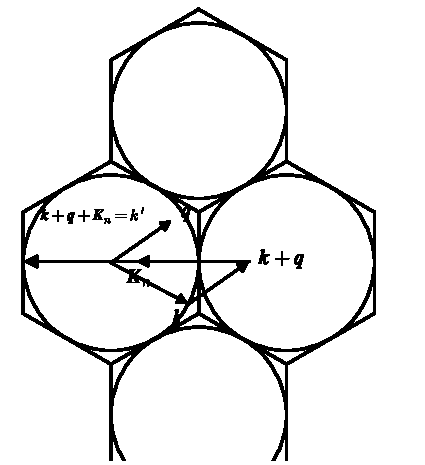
\includegraphics[width=7cm]{fig5-4.pdf}\\{\small 图 5.4\quad U 过程}
\end{minipage}
\end{center}

实际上在 BZ 之外，$\boldsymbol{k}+\boldsymbol{q}$ 处电子的速度与简约区内 $\boldsymbol{k}'=\boldsymbol{k}+\boldsymbol{q}+\boldsymbol{K}_n$ 点电子速度相同，它们都垂直于图中绘出的球形等能面.比较 $\boldsymbol{v}\left(\boldsymbol{k}\right)$ 和 $\boldsymbol{v}\left(\boldsymbol{k}+\boldsymbol{q}\right)$ 或 $\boldsymbol{v}\left(\boldsymbol{k}+\boldsymbol{q}+\boldsymbol{K}_n\right)$，显然散射前后电子速度发生了大角度偏转，好像经过了翻转，故常称 $\boldsymbol{K}_n\neq 0$ 的过程为 U 过程或倒逆过程.图5.5是 U 过程散射前后能带电子速度的变化，其中 $\boldsymbol{k}'=\boldsymbol{k}+\boldsymbol{q}+\boldsymbol{K}_n$ 代表散射后电子的简约波矢，而 $\boldsymbol{k}+\boldsymbol{q}$ 为不采用简约区方案时的散射波矢.由于在两种情况下速度相同，说明采用简约区方案划分 N 与 U 过程并不改变物理实质，仅仅是为了处理问题方便.

\begin{center}
\begin{minipage}{7.5cm}
\centering
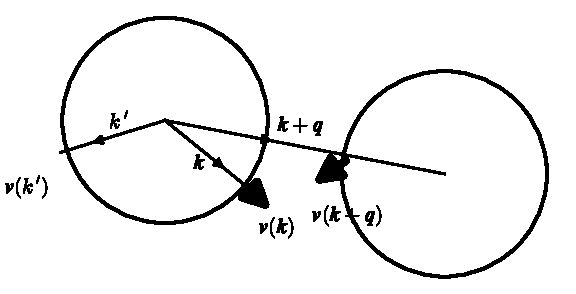
\includegraphics[width=7.5cm]{fig5-5.pdf}\\{\small 图 5.5\quad U 过程散射的电子速度图}
\end{minipage}
\end{center}

U 过程对于金属的高温特性有重要影响，因为在高温时大 $\boldsymbol{q}$ 值的散射过程增多，这时 $\boldsymbol{k}+\boldsymbol{q}$ 超出第一布里渊区的机会也多，于是 U 过程出现的概率增大.在低温下，当长波近似适用时，主要是 N 过程.

现在讨论电子-声子互作用过程的守恒律.由于 $H_{\mathrm{ep}}$ 只含声子产生及消灭算符的一次项，因此每次相互作用电子只可能吸收或发射一个声子.根据式(5.2.20)电子与声子的散射过程满足准动量关系
\begin{equation}
  \hbar\boldsymbol{k}'=\hbar\left(\boldsymbol{k}+\boldsymbol{q}+\boldsymbol{K}_n\right)
\end{equation}
显然，总动量守恒条件相差 $\hbar\boldsymbol{K}_n$，这是晶体结构的周期性和不连续性所造成的.假如完全忽略晶体的结构，则晶格求和 $\frac{1}{N}\sum\limits_{l}\mathrm{e}^{\mathrm{i}\left(\boldsymbol{k}+\boldsymbol{q}-\boldsymbol{k}'\right)\cdot\boldsymbol{l}}$ 过渡为连续积分
\begin{equation}
  \left(\frac{1}{N\Omega}\right)\int\mathrm{d}\boldsymbol{r}\;
  \mathrm{e}^{\mathrm{i}\left(\boldsymbol{k}+\boldsymbol{q}-\boldsymbol{k}'\right)\cdot\boldsymbol{r}}
  =\delta_{k',\,k+q}
\end{equation}
满足严格的动量守恒条件.这相当于假定晶体对无限小位移具有平移不变性，即正格矢 $\boldsymbol{a}_i\to 0$ 时，倒格矢 $\boldsymbol{b}_i\to\infty$，第一布里渊区变为无限大，也就不存在 $\boldsymbol{k}+\boldsymbol{q}$ 超出 BZ 的问题了.所以，一旦计及了晶体结构的影响，就会出现差 $\hbar\boldsymbol{K}_n$ 的准动量守恒条件，这是固体中元激发的特征.

讨论电子-声子散射过程的能量关系时，要区分实过程（可观测的）与虚过程（不可观测的）.先讨论实过程，根据含时微扰理论，从电子-声子系统的初态 $\left|i\right\rangle$ 到终态 $\left|f\right\rangle$ 的跃迁概率为
\begin{equation}
\begin{aligned}
  W\left(i\to f\right)&=\frac{2\pi}{\hbar}\left|\left\langle f\middle|H_{\mathrm{ep}}\middle|i\right\rangle\right|^2
  \frac{\sin^{2}\left(\dfrac{E_f-E_i}{2\hbar}\right)t}{\pi\left(\dfrac{t}{2\hbar}\right)\left(E_f-E_i\right)^2}\\
  &\overset{(t\ \text{大时})}{\Longrightarrow}\ \frac{2\pi}{\hbar}
  \left|\left\langle f\middle|H_{\mathrm{ep}}\middle|i\right\rangle\right|^2\delta\left(E_f-E_i\right)
\end{aligned}
\end{equation}
其中
\begin{equation}
  E_f-E_i=\varepsilon_{k'}-\varepsilon_k\mp\hbar\omega_{\pm q}
  \text{，}\quad \boldsymbol{k}'=\boldsymbol{k}+\boldsymbol{q}+\boldsymbol{K}_n
\end{equation}
若把电子与声子看作两个相互作用的子系统，则只有当我们能够确定电子从初态到终态的能量变化 $\Delta E=\left|\varepsilon_k-\varepsilon_{k'}\right|$ 时，这一跃迁才是可能的.按照不确定关系，这时应要求 $t\gg\hbar/\Delta E$ 才能将式(5.2.27)写成 $\delta$ 函数.又因为对于电子-声子散射过程，$t$ 最长只能取发生两次相继散射的平均间隔时间 $\tau$（弛豫时间），即 $t\leqslant\tau$.由此可知，只有当电子-声子散射的弛豫时间满足条件
\begin{equation*}
  \tau\gg\frac{\hbar}{\Delta E}\text{，}\qquad \Delta E=\left|\varepsilon_k-\varepsilon_{k+q}\right|
\end{equation*}
时才能得到
\begin{equation}
  W\left(i\to f\right)=\frac{2\pi}{\hbar}\left|\left\langle f\middle|H_{\mathrm{ep}}\middle|i\right\rangle\right|^2
  \delta\left(E_f-E_i\right)
\end{equation}
上式说明散射前后总能量守恒.参考式(5.2.28)，能量守恒条件为
\begin{equation}
  \varepsilon_{k'}=\varepsilon_{k+q}=\varepsilon_k\pm\hbar\omega_{\pm q}=\varepsilon_k\pm\hbar\omega_q
\end{equation}
式(5.2.30)对于 N 过程和 U 过程都一样，因为当电子在同一能带中发生跃迁时，$\varepsilon_{k+q}=\varepsilon_{k+q+\boldsymbol{K}_n}=\varepsilon_{k'}$.此外，在式(5.2.30)中还应用了时间反演对称性 $\omega_{-q}=\omega_q$.

由此不难求得电子从 $\boldsymbol{k}$ 态到 $\boldsymbol{k}+\boldsymbol{q}$ 的 N 过程跃迁概率为
\begin{equation}
\begin{aligned}
  W\left(\boldsymbol{k}\to\boldsymbol{k}+\boldsymbol{q}\right)&=\frac{2\pi}{\hbar}\left|D_q\right|^2
  \bigl\{\delta\left(\varepsilon_{k+q}-\varepsilon_k-\hbar\omega_q\right)\times\\
  &\quad\left|\left\langle n_{k+q}+1,n_k-1;n_q-1,n_{-q}\middle|a_qC_{k+q}^{+}C_k
  \middle|n_{k+q},n_k;n_q,n_{-q}\right\rangle\right|^2+\\
  &\quad\delta\left(\varepsilon_{k+q}-\varepsilon_k+\hbar\omega_q\right)\times\\
  &\quad\left|\left\langle n_{k+q}+1,n_k-1;n_q,n_{-q}+1\middle|a_{-q}^{+}C_{k+q}^{+}C_k
  \middle|n_{k+q},n_k;n_q,n_{-q}\right\rangle\right|^2\bigl\}\\
  &=\frac{2\pi}{\hbar}\left|D_q\right|^2\left(1-n_{k+q}\right)n_k
  \bigl\{n_q\delta\left(\varepsilon_{k+q}-\varepsilon_k-\hbar\omega_q\right)+\\
  &\quad\left(n_{-q}+1\right)\delta\left(\varepsilon_{k+q}-\varepsilon_k+\hbar\omega_q\right)\bigr\}
\end{aligned}
\end{equation}
以上结果仅仅涉及电子从已占据态 $\left(n_k=1\right)$ 向空占态 $\left(n_{k+q}=0\right)$ 的跃迁，因此在第一个等号右边的状态中，$\left(n_{k+q}+1\right)$ 与 $\left(n_k-1\right)$ 实际上分别为 1 与 0 占据，符合电子系统的泡利原理，而第二个等号右边的因子 $\left(1-n_{k+q}\right)n_k$ 在此情形下实际上等于 1.在这里保留该因子的目的是为了将以上结果推广用于 $T>0$ 情形，这时只需将 $n_k$ 与 $n_q$ 等分别用费密与玻色分布代替，即可将上式推广用于计算有限温度时电子与声子散射的弛豫时间，给出正确的电阻温度关系.

\section{声子的自能修正}

现在利用电子与声子互作用的集体坐标表示式(5.2.24)计算 LA 声子的自能修正.考虑单价金属，设 $N$ 个离子组成的简单晶格浸没在均匀电子气体中.与电子集体振荡相类似，在此模型中未微扰的 LA 声子频率在长波范围内可用离子的等离子集体振荡频率表示
\begin{equation}
  \Omega_q^2=\frac{4\pi Ne^2}{M}
\end{equation}
这里晶体取单位体积，$N=\Omega^{-1}$，$\Omega$ 为正点阵元胞体积.将上式代入式(2.4.3)，得到 LA 声子的哈密顿量
\begin{equation}
  H_{\mathrm{p}}=\frac{1}{2}\sum_{q}\left\{P_{-q}P_q+\Omega_q^2Q_{-q}Q_q\right\}
\end{equation}
其中 $P_{-q}=\dot{Q}_q$.电子与声子互作用为
\begin{equation*}
  H_{\mathrm{ep}}=\sum_{q}M_qQ_q\rho_{-q}
\end{equation*}
金属的总哈密顿量
\begin{equation}
  H=H_{\mathrm{p}}+H_{\mathrm{ep}}+H_{\mathrm{e}}+H_{\mathrm{ee}}
\end{equation}
其中 $H_{\mathrm{e}}$ 为自由电子近似的哈密顿量，$H_{\mathrm{ee}}$ 代表电子之间的库仑互作用，这两项均与声子的简正坐标 $Q_q$ 无关.

根据海森伯方程 $\mathrm{i}\hbar\dot{P}_{-q}=\left[P_{-q},H\right]$ 和对易式 $\left[P_q,Q_{q'}\right]=\dfrac{\hbar}{\mathrm{i}}\delta_{qq'}$，立刻可导出 $Q_q$ 的运动方程
\begin{equation}
  \ddot{Q}_q+\Omega_q^2Q_q=-M_{-q}\rho_q
\end{equation}
其中
\begin{equation}
  M_{-q}=-\mathrm{i}\left(\frac{N}{M}\right)^{1/2}\frac{4\pi e^2}{q^2}
  \left(\boldsymbol{e}_q\cdot\boldsymbol{q}\right)
\end{equation}
如果能确定式(5.3.4)右边的 $\rho_q$ 与 $Q_q$ 之间的关系，则声子频率的修正就可以求出.

由于晶格振动必然产生离子密度的起伏，可用离子密度的傅里叶分量 $\rho_q^{\mathrm{i}}$ 描述.这个起伏的效果相当于对电子气体加上外扰动场，它将引起电子气体的响应运动，从而使均匀分布的电子气产生密度起伏 $\rho_q$.所以，首先应找出 $\rho_q^{\mathrm{i}}$ 与简正坐标的关系，然后再利用线性响应理论决定 $\rho_q$ 与 $\rho_q^{\mathrm{i}}$ 的关系.

\subsection*{(i) 离子密度起伏 $\rho_q^{\mathrm{i}}$}

晶格振动位移将产生极化
\begin{equation}
\begin{aligned}
  \boldsymbol{P}\left(\boldsymbol{r}\right)&=Ne\,\boldsymbol{u}\left(\boldsymbol{r}\right)\\
  \boldsymbol{u}\left(\boldsymbol{r}\right)&=\left(NM\right)^{-1/2}\sum_{q}\boldsymbol{e}_qQ_q\mathrm{e}^{\mathrm{i}\boldsymbol{q}\cdot\boldsymbol{r}}
\end{aligned}
\end{equation}
由极化可得到离子密度
\begin{equation}
  \rho^{\mathrm{i}}\left(\boldsymbol{r}\right)=-\frac{1}{e}\nabla\cdot\boldsymbol{P}\left(\boldsymbol{r}\right)
  =-\mathrm{i}\left(\frac{N}{M}\right)^{1/2}\sum_{q}\left(\boldsymbol{e}_q\cdot\boldsymbol{q}\right)Q_q\mathrm{e}^{\mathrm{i}\boldsymbol{q}\cdot\boldsymbol{r}}
\end{equation}
再将 $\rho^{\mathrm{i}}\left(\boldsymbol{r}\right)$ 展开为傅里叶级数
\begin{equation}
  \rho^{\mathrm{i}}\left(\boldsymbol{r}\right)=\sum_{q}\rho_q^{\mathrm{i}}\mathrm{e}^{\mathrm{i}\boldsymbol{q}\cdot\boldsymbol{r}}
\end{equation}
即得离子密度的傅里叶分量
\begin{equation}
  \rho_q^{\mathrm{i}}=-\mathrm{i}\left(\frac{N}{M}\right)^{1/2}\left(\boldsymbol{e}_q\cdot\boldsymbol{q}\right)Q_q
\end{equation}

\subsection*{(ii) $\rho_q$ 与 $\rho_q^{\mathrm{i}}$ 的关系}

由于离子运动比电子慢得多，因此可将离子运动产生的 $\rho_q^{\mathrm{i}}$ 当作“静态的试探电荷”，并用线性响应理论处理.这时有
\begin{equation}
  \left.\begin{aligned}
  \nabla\cdot\boldsymbol{D}&=4\pi e\rho^{\mathrm{i}}\left(\boldsymbol{r}\right)\\
  \nabla\cdot\boldsymbol{E}&=4\pi e\left\{\rho^{\mathrm{i}}\left(\boldsymbol{r}\right)-\rho\left(\boldsymbol{r}\right)\right\}
  \end{aligned}\right\}
\end{equation}
$\rho\left(\boldsymbol{r}\right)$ 为电子气体的密度，令
\begin{equation}
  \left.\begin{aligned}
  \boldsymbol{D}\left(\boldsymbol{r}\right)&=\sum_{q}\boldsymbol{D}\left(\boldsymbol{q}\right)\mathrm{e}^{\mathrm{i}\boldsymbol{q}\cdot\boldsymbol{r}}\\
  \boldsymbol{E}\left(\boldsymbol{r}\right)&=\sum_{q}\boldsymbol{E}\left(\boldsymbol{q}\right)\mathrm{e}^{\mathrm{i}\boldsymbol{q}\cdot\boldsymbol{r}}\\
  \boldsymbol{D}\left(\boldsymbol{q}\right)&=\varepsilon\left(\boldsymbol{q}\right)\boldsymbol{E}\left(\boldsymbol{q}\right)
  \end{aligned}\right\}
\end{equation}
则可以通过静态介电函数 $\varepsilon\left(\boldsymbol{q}\right)$ 决定电子密度起伏.由式(5.3.10)与(5.3.11)可得到
\begin{equation}
\begin{aligned}
  4\pi e\rho_q^{\mathrm{i}}&=\mathrm{i}\boldsymbol{q}\cdot\boldsymbol{D}\left(\boldsymbol{q}\right)
  =\mathrm{i}\varepsilon\left(\boldsymbol{q}\right)\boldsymbol{q}\cdot\boldsymbol{E}\left(\boldsymbol{q}\right)\\
  &=\varepsilon\left(\boldsymbol{q}\right)4\pi e\left(\rho_q^{\mathrm{i}}-\rho_q\right)
\end{aligned}
\end{equation}
于是
\begin{equation}
  \rho_q=-\frac{1-\varepsilon\left(\boldsymbol{q}\right)}{\varepsilon\left(\boldsymbol{q}\right)}\rho_q^{\mathrm{i}}
\end{equation}
再利用式(5.3.5)和式(5.3.9)，求得运动方程式(5.3.4)右边的
\begin{equation}
\begin{aligned}
  M_{-q}\rho_q&=\frac{4\pi Ne^2}{M}\cdot\frac{\left(\boldsymbol{e}_q\cdot\boldsymbol{q}\right)^2}{q^2}
  \cdot\frac{1-\varepsilon\left(\boldsymbol{q}\right)}{\varepsilon\left(\boldsymbol{q}\right)}\,Q_q\\
  &=\Omega_q^2\ \frac{1-\varepsilon\left(\boldsymbol{q}\right)}{\varepsilon\left(\boldsymbol{q}\right)}\,Q_q
\end{aligned}
\end{equation}
这样计及了电子气体的屏蔽作用后，LA 声子的运动方程为
\begin{equation}
  \ddot{Q}_q+\frac{\Omega_q^2}{\varepsilon\left(\boldsymbol{q}\right)}Q_q=0
\end{equation}
由此求出 LA 声子的频率
\begin{equation}
  \omega_q^2=\Omega_q^2/\varepsilon\left(\boldsymbol{q}\right)
\end{equation}
若取托马斯-费密介电函数式(4.8.3)
\begin{equation}
  \varepsilon\left(\boldsymbol{q}\right)=1+\frac{\lambda^2}{q^2}
  \text{，}\ \lambda^2=\frac{6\pi Ne^2}{E_{\mathrm{F}}}
\end{equation}
则在长波范围内
\begin{equation}
  \omega_q^2=\Omega_q^2\frac{q^2}{q^2+\lambda^2}
  \approx\Omega_q^2\frac{q^2}{\lambda^2}
  =\frac{1}{3}\left(\frac{m}{M}\right)v_{\mathrm{F}}^2q^2
\end{equation}
最后得到 LA 声子的色散关系为
\begin{equation}
  \omega_q=c_{\mathrm{L}}q
\end{equation}
\begin{equation}
  c_{\mathrm{L}}=\left(\frac{1}{3}\ \frac{m}{M}\right)^{1/2}v_{\mathrm{F}}
\end{equation}
其中 $v_{\mathrm{F}}=\hbar k_{\mathrm{F}}/m$ 为费密速度.这就是著名的玻姆-司台夫（Bohm-Staver）声速公式\textsuperscript{[3]}.

\section{电子与光频声子的相互作用}

根据第二章§6的讨论，我们已经知道离子晶体中的光频支纵振动会产生极化电场.这个电场除了使 LO 声子的频率高于 TO 声子的频率以外，还将对离子晶体中的传导电子产生强烈的耦合作用，它比 LA 声子（代表质心运动，不产生极化电场）对传导电子的作用强得多.因此，主要是 LO 声子与传导电子的相互作用对离子晶体中的载流子特性产生影响.

在长波近似下，LO 声子的位移场可写为
\begin{equation}
\begin{aligned}
  \boldsymbol{u}_{+}\left(\boldsymbol{r}\right)-\boldsymbol{u}_{-}\left(\boldsymbol{r}\right)
  &=\frac{1}{\sqrt{NM}}\sum_{q}\boldsymbol{e}_qQ_q\mathrm{e}^{\mathrm{i}\boldsymbol{q}\cdot\boldsymbol{r}}\\
  &=\sqrt{\frac{\hbar}{2NM\omega_{\mathrm{L}}}}\sum_{q}\boldsymbol{e}_q
  \left(a_q\mathrm{e}^{\mathrm{i}\boldsymbol{q}\cdot\boldsymbol{r}}+a_q^{+}\mathrm{e}^{-\mathrm{i}\boldsymbol{q}\cdot\boldsymbol{r}}\right)
\end{aligned}
\end{equation}
其中 $M$ 为折合质量，对于 NaCl 和 CsCl 等离子晶体，$M=\dfrac{M_+M_-}{M_++M_-}$.式(5.4.1)中还忽略了 $\omega_{\mathrm{L}}$ 对 $\boldsymbol{q}$ 的依赖关系，近似取 $\boldsymbol{q}=0$ 时的 $\omega_{\mathrm{L}}$ 值.

根据式(2.6.24)纵振动位移所产生的电场
\begin{equation}
  \boldsymbol{E}\left(\boldsymbol{r}\right)=-\frac{4\pi\gamma_{12}}{1+4\pi\gamma_{22}}\boldsymbol{W}\left(\boldsymbol{r}\right)
\end{equation}
并按照式(2.6.1)和设晶体的体积 $V=N\Omega=1$，得到
\begin{equation}
\begin{aligned}
  \boldsymbol{W}\left(\boldsymbol{r}\right)&=\sqrt{NM}\left\{\boldsymbol{u}_{+}\left(\boldsymbol{r}\right)
  -\boldsymbol{u}_{-}\left(\boldsymbol{r}\right)\right\}\\
  &=\sqrt{\frac{\hbar}{2\omega_{\mathrm{L}}}}\sum_{q}\boldsymbol{e}_q
  \left(a_q\mathrm{e}^{\mathrm{i}\boldsymbol{q}\cdot\boldsymbol{r}}+a_q^{+}\mathrm{e}^{-\mathrm{i}\boldsymbol{q}\cdot\boldsymbol{r}}\right)
\end{aligned}
\end{equation}
LO 声子的极化电场可写成
\begin{equation}
  \boldsymbol{E}\left(\boldsymbol{r}\right)=-4\pi F\sum_{q}\boldsymbol{e}_q
  \left(a_q\mathrm{e}^{\mathrm{i}\boldsymbol{q}\cdot\boldsymbol{r}}+a_q^{+}\mathrm{e}^{-\mathrm{i}\boldsymbol{q}\cdot\boldsymbol{r}}\right)
\end{equation}
其中常量 $F$ 由 LST 关系式(2.6.27)和 $\gamma_{ij}$ 的公式(2.6.18)定出为
\begin{equation}
  F=\left\{\frac{\hbar\omega_{\mathrm{L}}}{8\pi}\left(\frac{1}{\varepsilon_{\infty}}-\frac{1}{\varepsilon_0}\right)\right\}^{1/2}
\end{equation}
若设电场的势
\begin{equation}
  \varphi\left(\boldsymbol{r}\right)=\sum_{q}\left(\varphi_q\mathrm{e}^{\mathrm{i}\boldsymbol{q}\cdot\boldsymbol{r}}
  +\varphi_q^{+}\mathrm{e}^{-\mathrm{i}\boldsymbol{q}\cdot\boldsymbol{r}}\right)
\end{equation}
则由
\begin{equation}
  \boldsymbol{E}\left(\boldsymbol{r}\right)=-\nabla\varphi\left(\boldsymbol{r}\right)
  =-\mathrm{i}\sum_{q}\boldsymbol{q}\left(\varphi_q\mathrm{e}^{\mathrm{i}\boldsymbol{q}\cdot\boldsymbol{r}}
  -\varphi_q^{+}\mathrm{e}^{-\mathrm{i}\boldsymbol{q}\cdot\boldsymbol{r}}\right)
\end{equation}
与式(5.4.4)相比较求得
\begin{equation}
  \left.\begin{aligned}
  \varphi_q&=-\mathrm{i}\frac{4\pi F}{q^2}\left(\boldsymbol{e}_q\cdot\boldsymbol{q}\right)a_q\\
  \varphi_q^{+}&=\mathrm{i}\frac{4\pi F}{q^2}\left(\boldsymbol{e}_q\cdot\boldsymbol{q}\right)a_q^{+}
  \end{aligned}\right\}
\end{equation}
因此
\begin{equation}
  \varphi\left(\boldsymbol{r}\right)=-\mathrm{i}4\pi F\sum_{q}\frac{\boldsymbol{e}_q\cdot\boldsymbol{q}}{q^2}
  \left(a_q\mathrm{e}^{\mathrm{i}\boldsymbol{q}\cdot\boldsymbol{r}}-a_q^{+}\mathrm{e}^{-\mathrm{i}\boldsymbol{q}\cdot\boldsymbol{r}}\right)
\end{equation}
$-e\varphi\left(\boldsymbol{r}\right)$ 代表 $\boldsymbol{r}$ 处电子受 LO 声子作用的势能，也就是电子与 LO 声子的相互作用，因此
\begin{equation}
\begin{aligned}
  H_{\mathrm{ep}}&=-e\int\varPsi^{+}\left(\boldsymbol{r}\right)\varphi\left(\boldsymbol{r}\right)\varPsi\left(\boldsymbol{r}\right)\mathrm{d}\boldsymbol{r}\\
  &=\mathrm{i}4\pi eF\sum_{k,k',q}\frac{\boldsymbol{e}_q\cdot\boldsymbol{q}}{q^2}
  \bigg(a_qC_{k'}^{+}C_k\int\mathrm{e}^{\mathrm{i}\left(\boldsymbol{k}+\boldsymbol{q}-\boldsymbol{k}'\right)\cdot\boldsymbol{r}}
  u_{k'}^{*}\left(\boldsymbol{r}\right)u_k\left(\boldsymbol{r}\right)\mathrm{d}\boldsymbol{r}\,-\\
  &\quad a_q^{+}C_{k'}^{+}C_k\int\mathrm{e}^{\mathrm{i}\left(\boldsymbol{k}-\boldsymbol{q}-\boldsymbol{k}'\right)\cdot\boldsymbol{r}}
  u_{k'}^{*}\left(\boldsymbol{r}\right)u_k\left(\boldsymbol{r}\right)\mathrm{d}\boldsymbol{r}\bigg)
\end{aligned}
\end{equation}
当 $u_k\left(\boldsymbol{r}\right)$ 取自由电子近似时，对于 N 过程
\begin{equation}
  H_{\mathrm{ep}}=\mathrm{i}4\pi eF\sum_{k,q}\frac{\boldsymbol{e}_q\cdot\boldsymbol{q}}{q^2}
  \left(a_qC_{k+q}^{+}C_k-a_q^{+}C_{k-q}^{+}C_k\right)
\end{equation}
现在利用上式计算 $H_{\mathrm{ep}}$ 对电子自能的修正.当电子在离子晶体中运动时，将使周围的正、负离子产生相对位移，形成介质的局域极化.由于极化伴随着电子运动，因此在介质中将激发 LO 声子.这样，电子带着晶格极化运动，就像带着声子运动一样，必将改变电子的基态能量和有效质量，使之成为一个（电子+极化）的实体，称为极化子（polaron），极化子是电子与 LO 声子相耦合系统的准粒子.当极化的范围比晶格常数大很多时，称为大极化子，反之称为小极化子.对于大极化子可采用连续模型，其理论发展也较完善.下面介绍弗留里希（H.Fr\"{o}hlich）等人的微扰处理，这是场论方法用于固体的第一项工作\textsuperscript{[4]}.

设导带底部 $\left|\boldsymbol{k}\right\rangle$ 状态上有一个电子，其能量为
\begin{equation}
  \varepsilon_k=\frac{\hbar^2k^2}{2m}<\hbar\omega_{\mathrm{L}}
\end{equation}
称为慢电子，其中 $m$ 为能带电子的有效质量，当 $T=0$ K 时声子处于真空态 $\left|0\right\rangle$，故不计互作用时系统的状态为
\begin{equation}
  \left|\boldsymbol{k};0\right\rangle=\left|\boldsymbol{k}\right\rangle\left|0\right\rangle
  =\left|\boldsymbol{k}\right\rangle\prod_{q}\left|0_q\right\rangle
\end{equation}
设电子与声子的相互作用比较弱，则可用微扰论计算 $H_{\mathrm{ep}}$ 对电子状态和能量的修正.
\begin{equation}
  \left|\boldsymbol{k};0\right\rangle_1=\left|\boldsymbol{k};0\right\rangle+\sum_{q}
  \frac{\left\langle \boldsymbol{k}-\boldsymbol{q};1_q\middle|H_{\mathrm{ep}}\middle|\boldsymbol{k};0_q\right\rangle}
  {\varepsilon_k-\varepsilon_{k-q}-\hbar\omega_{\mathrm{L}}}
  \left|\boldsymbol{k}-\boldsymbol{q};1_q\right\rangle
\end{equation}
代表准至 $H_{\mathrm{ep}}$ 一阶的波函数.这里考虑到初态为声子真空，因此只计算发射声子的矩阵元.准至二阶的电子能量为
\begin{equation}
  E_k=\varepsilon_k+\sum_{q}
  \frac{\left|\left\langle \boldsymbol{k}-\boldsymbol{q};1_q\middle|H_{\mathrm{ep}}\middle|\boldsymbol{k};0_q\right\rangle\right|^2}
  {\varepsilon_k-\varepsilon_{k-q}-\hbar\omega_{\mathrm{L}}}
\end{equation}
上式与图5.3(a)相对应，它代表电子先发射 $\boldsymbol{q}$ 声子，然后再吸收同一声子的自能过程，其中应限制能量分母 $\left(\varepsilon_k-\varepsilon_{k-q}-\hbar\omega_{\mathrm{L}}\right)\neq 0$.由于
\begin{equation}
\begin{aligned}
  a_qC_k^{+}C_{k-q}\left|\boldsymbol{k}-\boldsymbol{q};\ 1_q\right\rangle&=\left|\boldsymbol{k};\ 0_q\right\rangle\\
  a_q^{+}C_{k-q}^{+}C_k\left|\boldsymbol{k};\ 0_q\right\rangle&=\left|\boldsymbol{k}-\boldsymbol{q};\ 1_q\right\rangle\\
  \left\langle \boldsymbol{k};\ 0_q\middle|\boldsymbol{k};\ 0_q\right\rangle
  &=\left\langle \boldsymbol{k}-\boldsymbol{q};\ 1_q\middle|\boldsymbol{k}-\boldsymbol{q};\ 1_q\right\rangle=1
\end{aligned}
\end{equation}
可求得式(5.4.15)分子为
\begin{equation}
  \left|\left\langle \boldsymbol{k}-\boldsymbol{q};\ 1_q\middle|H_{\mathrm{ep}}\middle|\boldsymbol{k};\ 0_q\right\rangle\right|^2
  =\left(\frac{4\pi eF}{q}\right)^2
\end{equation}
因此
\begin{equation*}
\begin{aligned}
  E_k&=\varepsilon_k+\sum_{q}\left(\frac{4\pi eF}{q}\right)^2
  \frac{1}{\varepsilon_k-\varepsilon_{k-q}-\hbar\omega_{\mathrm{L}}}\\
  &=\frac{\hbar^2k^2}{2m}-\frac{\left(4\pi eF\right)^2}{\left(2\pi\right)^3}\left(\frac{2m}{\hbar^2}\right)
  \int\frac{\mathrm{d}^3q}{q^2}\,
  \frac{1}{\Bigl[q^2+\Bigl(\frac{2m\omega_{\mathrm{L}}}{\hbar}\Bigr)-2\boldsymbol{k}\cdot\boldsymbol{q}\Bigr]}
\end{aligned}
\end{equation*}
对于慢电子 $\boldsymbol{k}$ 很小，可将被积函数按 $\boldsymbol{k}$ 展开到二级，再考虑到被积函数随 $\boldsymbol{q}$ 增大快速下降，积分的上限可取 $q=\infty$.最后算出
\begin{equation}
  E_k=-\alpha\hbar\omega_{\mathrm{L}}+\frac{\hbar^2k^2}{2m}
  \left(1-\frac{\alpha}{6}\right)+\cdots
\end{equation}
其中量纲为 1 的耦合常数
\begin{equation}
\begin{aligned}
  \alpha&\equiv\frac{\left(4\pi eF\right)^2}{\left(2\pi\right)^3\hbar\omega_{\mathrm{L}}}
  \left(\frac{2m}{\hbar^2}\right)\int\frac{\mathrm{d}^3q}{q^2}\,
  \frac{1}{\Bigl[\ q^2+\Bigl(\frac{2m\omega_{\mathrm{L}}}{\hbar}\Bigr)\Bigr]}\\
  &=\frac{16m}{\hbar^3\omega_{\mathrm{L}}}\,F^2e^2\int_{0}^{\infty}
  \frac{\mathrm{d}q}{q^2+\Bigl(\frac{2m\omega_{\mathrm{L}}}{\hbar}\Bigr)}\\
  &=\frac{e^2}{2\hbar\omega_{\mathrm{L}}}\left(\frac{2m\omega_{\mathrm{L}}}{\hbar}\right)^{1/2}
  \left(\frac{1}{\varepsilon_{\infty}}-\frac{1}{\varepsilon_0}\right)
\end{aligned}
\end{equation}
式(5.4.18)说明电子与 LO 声子的相互作用使导带的带边能量降低 $\alpha\hbar\omega_{\mathrm{L}}$，而有效质量则相应地增大
\begin{equation}
  m^{*}=\frac{m}{1-\alpha/6}
\end{equation}
$m^{*}$ 称为极化子的有效质量，$E_k$ 为极化子能量.

利用式(5.4.14)还可以计算在电子周围所激发的平均声子数
\begin{equation}
\begin{aligned}
  \left\langle N_{\text{声}}\right\rangle&={}_1\left\langle \boldsymbol{k};0\middle|
  \sum_{q}a_q^{+}a_q\middle|\boldsymbol{k};0\right\rangle_1\\
  &=\sum_{q}\frac{\left|\left\langle \boldsymbol{k}-\boldsymbol{q};1_q\middle|H_{\mathrm{ep}}
  \middle|\boldsymbol{k};0_q\right\rangle\right|^2}
  {\left(\varepsilon_k-\varepsilon_{k-q}-\hbar\omega_{\mathrm{L}}\right)^2}
\end{aligned}
\end{equation}
对于慢电子可令上式中 $\boldsymbol{k}\to 0$，求得
\begin{equation}
  \left\langle N_{\text{声}}\right\rangle=\frac{\left(4\pi eF\right)^2}{\left(2\pi\right)^3}\,
  4\pi\left(\frac{2m}{\hbar^2}\right)^2\int_{0}^{\infty}
  \frac{\mathrm{d}q}{\Bigl[\ q^2+\Bigl(\frac{2m\omega_{\mathrm{L}}}{\hbar}\Bigr)\Bigr]^2}=\frac{\alpha}{2}
\end{equation}
式(5.4.22)说明极化子中的平均声子数与量纲为 1 的耦合常数 $\alpha$ 成正比.这里存在一个待说明的新概念.由于我们是在 $T=0$ K 时讨论电子-声子互作用问题.这时既没有热声子激发，并且还假定了电子的能量 $\frac{\hbar^2k^2}{2m}$ 小于声子能量 $\hbar\omega_{\mathrm{L}}$.因此，在以上讨论中谈到的“电子发射声子”过程不可能是实过程，因为它不满足能量守恒原理.但是，假如过程发生的时间 $\Delta t$ 足够短，根据测不准关系，$\Delta E\sim\hbar/\Delta t$ 可以相当大，以至于超过 $\hbar\omega_{\mathrm{L}}$，从而发射声子，这样的声子称为虚声子（virtual phonon）\nobreak.由于 $\Delta t$ 很短，虚声子不可能被测得，它只不过是电子带着周围的晶格极化运动的场论说法而已！因此，$\langle N_{\text{声}}\rangle$ 代表电子周围的平均虚声子数.类似的，图5.3(a)［或二级微扰能量算式(5.4.15)］应当解释为：$\boldsymbol{k}$ 电子先发射 $\boldsymbol{q}$ 虚声子到达中间态 $\boldsymbol{k}-\boldsymbol{q}$，然后再吸收此虚声子回到原来状态，电子在中间态所停留的时间极短，不可能被测出，这样的过程称为虚过程或中间过程.

最后指出，用微扰方法求得的极化子能量公式(5.4.18)只适用于 $\alpha\ll 1$ 情况，否则微扰失效.但是大多数离子晶体的 $\alpha$ 值都大于 1（见表5.1），只有少数 Ⅲ-Ⅴ 族和 Ⅱ-Ⅵ 族化合物半导体 $\alpha\ll 1$.因此，极化子问题是强耦合问题，一般不能用微扰方法处理.我们将在第八章中详细介绍极化子的非微扰理论.

\begin{center}
\textbf{表 5.1\quad 离子晶体的耦合常数}\\[0.8em]
\begin{tabular}{|c|c||c|c|}
\hline
离子晶体 & 耦合常数 $\alpha$ & 离子晶体 & 耦合常数 $\alpha$\\\hline
KI & 7.8 & CuCl & 3.4\\\hline
CsCl & 6.4 & LiI & 2.4\\\hline
KCl & 5.9 & MgO & 2.4\\\hline
NaCl & 5.5 & ZnS & 1.3\\\hline
NaI & 4.8 & CdS & 0.65\\\hline
AgCl & 4.2 & InP & 0.08\\\hline
AgBr & 4.1 & InSb & 0.013\\\hline
\end{tabular}
\end{center}

\section{有效电子-电子相互作用}

在上一节中我们讨论了一个电子发射虚声子，然后又吸收它的过程.这种过程给出电子的自能修正，其物理实质是电子使晶格形变或极化，反过来这个形变或极化的势场又作用于同一电子，引起能谱的变化.现在讨论多电子系统与声子互作用情况，这时还可能发生另一种过程，一个电子发射的虚声子被另一个电子所吸收，从而产生电子与电子之间的有效相互作用.有效互作用的物理图像是十分明朗的，所谓电子发射虚声子，就是在这个电子周围产生了晶格形变或极化，假如另一个电子也走近形变区，它必将受吸引或排斥力的作用，但这不是电子间的直接库仑作用，而是一项全新的通过晶格振动传递的有效互作用.图5.6是有效互作用的示意图，它对应的互作用过程如图5.3(c).研究电子间通过交换虚声子所产生的有效互作用，对于解释超导电性的成因有重要意义.

\begin{center}
\begin{minipage}{7.5cm}
\centering
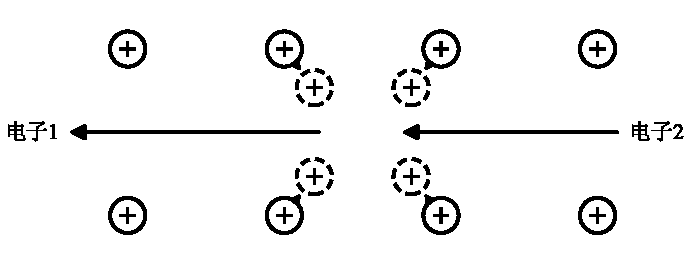
\includegraphics[width=7.5cm]{fig5-6.pdf}\\{\small 图 5.6\quad 电子-电子有效互作用}
\end{minipage}
\end{center}

我们讨论单价金属中电子与 LA 声子的互作用，根据式(5.2.22)其哈密顿量可写为
\begin{equation}
  \left.\begin{aligned}
  H_{\mathrm{ep}}&=\sum_{k,q,\sigma}\left(D_qa_qC_{k+q,\sigma}^{+}C_{k\sigma}
  +D_q^{+}a_q^{+}C_{k-q,\sigma}^{+}C_{k\sigma}\right)\\
  D_q&=-\mathrm{i}\left(\frac{N\hbar}{2M\omega_q}\right)^{1/2}V_q\left(\boldsymbol{e}_q\cdot\boldsymbol{q}\right)\\
  \boldsymbol{e}_{-q}=\boldsymbol{e}_q&\text{，}\ \omega_{-q}=\omega_q\text{，}\ \left|D_q\right|^2=\left|D_{-q}\right|^2
  \end{aligned}\right\}
\end{equation}
这里 $\sigma$ 为电子自旋，常用自旋朝上（$\uparrow$）或向下（$\downarrow$）表示，代表电子自旋在 $z$ 方向投影取 $\pm\dfrac{\hbar}{2}$ 值.为了图像清楚起见，我们先定性估计有效互作用的形式，然后再利用正则变换方法作较严格的推导.

\subsection*{1. 电子-电子有效互作用的微扰估计}

弗留里希\textsuperscript{[5]}首先利用二级玻恩散射矩阵对电子间交换 LA 声子的有效互作用进行了微扰估计，他按照下列图形所表示的两种虚声子过程（或中间过程）写出电子通过交换声子的互作用矩阵元为
\begin{equation}
\begin{aligned}
  &\sum_{m}\frac{\left\langle f\middle|H_{\mathrm{ep}}\middle|m\right\rangle
  \left\langle m\middle|H_{\mathrm{ep}}\middle|i\right\rangle}{E_i-E_m}\\
  &\quad=\sum_{q}\left|D_q\right|^2\biggl\{
  \frac{\left\langle f\middle|a_qC_{k+q,\sigma}^{+}C_{k\sigma}\middle|m_1\right\rangle
  \left\langle m_1\middle|a_q^{+}C_{k'-q,\sigma'}^{+}C_{k'\sigma'}\middle|i\right\rangle}
  {\varepsilon_{k'}-\varepsilon_{k'-q}-\hbar\omega_q}+\\
  &\qquad\frac{\left\langle f\middle|a_{-q}C_{k'-q,\sigma'}^{+}C_{k'\sigma'}\middle|m_2\right\rangle
  \left\langle m_2\middle|a_{-q}^{+}C_{k+q,\sigma}^{+}C_{k\sigma}\middle|i\right\rangle}
  {\varepsilon_k-\varepsilon_{k+q}-\hbar\omega_{-q}}\biggr\}
\end{aligned}
\end{equation}

\begin{center}
\begin{minipage}{8cm}
\centering
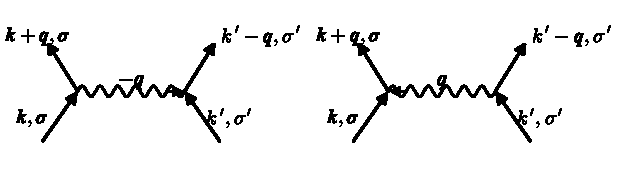
\includegraphics[width=8cm]{fig5-7.pdf}\\[0.3em]
{\small (a) $\boldsymbol{k}'$ 发射 $\boldsymbol{q}$ 声子\qquad\qquad (b) $\boldsymbol{k}$ 发射 $\left(-\boldsymbol{q}\right)$ 声子}\\[0.2em]
{\small 图 5.7\quad 电子-声子-电子互作用}
\end{minipage}
\end{center}

其中初态与终态
\begin{equation*}
\begin{aligned}
  &\left|i\right\rangle=\left|\cdots,\ n_{k\sigma},\ \cdots,\ n_{k'\sigma'},\ \cdots,\ n_{k'-q,\sigma'},\ \cdots,\ n_{k+q,\sigma},\ \cdots;\ 0\right\rangle\\
  &\left|f\right\rangle=\left|\cdots,\ \left(n_{k\sigma}-1\right),\ \cdots,\ \left(n_{k'\sigma'}-1\right),\ \cdots,\right.\\
  &\qquad\qquad\left.\left(n_{k'-q,\sigma'}+1\right),\ \cdots,\ \left(n_{k+q,\sigma}+1\right),\ \cdots;\ 0\right\rangle
\end{aligned}
\end{equation*}
为声子真空态，而两个中间态
\begin{equation*}
\begin{aligned}
  &\left|m_1\right\rangle=\left|\cdots,\ n_{k\sigma},\ \cdots,\ \left(n_{k'\sigma'}-1\right),\ \cdots,\right.\\
  &\qquad\qquad\left.\left(n_{k'-q,\sigma'}+1\right),\ \cdots,\ n_{k+q,\sigma},\ \cdots;\ 1_q\right\rangle\\
  &\left|m_2\right\rangle=\left|\cdots,\ \left(n_{k\sigma}-1\right),\ \cdots,\ n_{k'\sigma'},\ \cdots,\right.\\
  &\qquad\qquad\left.n_{k'-q,\sigma'},\ \cdots,\ \left(n_{k+q,\sigma}+1\right),\ \cdots;\ 1_{-q}\right\rangle
\end{aligned}
\end{equation*}
都有一个声子激发.$\left|m_1\right\rangle$ 与图5.7中(a)对应，$\left|m_2\right\rangle$ 与(b)对应.

利用 $\left\langle 1_q\middle|a_q^{+}\middle|0_q\right\rangle=\left\langle 0_q\middle|a_q\middle|1_q\right\rangle=1$，容易算出式(5.5.2)对声子态的平均.再考虑到散射前后能量守恒 $\varepsilon_k+\varepsilon_{k'}=\varepsilon_{k+q}+\varepsilon_{k'-q}$，可用 $\left(\varepsilon_{k+q}-\varepsilon_k\right)$ 代替第一项分母中的 $\left(\varepsilon_{k'}-\varepsilon_{k'-q}\right)$.这时两项分子的计算结果均与 $\left\langle f\middle|C_{k+q,\sigma}^{+}C_{k'-q,\sigma'}^{+}C_{k'\sigma'}C_{k\sigma}\middle|i\right\rangle$ 相等，因此，可以用一个不明显含声子算符的有效互作用矩阵元 $\left\langle f\middle|H_{\mathrm{eff}}\middle|i\right\rangle$ 代替式(5.5.2)，得
\begin{equation}
\begin{aligned}
  \left\langle f\middle|H_{\mathrm{eff}}\middle|i\right\rangle
  &=\sum_{q}\left|D_q\right|^2\biggl\{\frac{1}{\varepsilon_k-\varepsilon_{k+q}-\hbar\omega_{-q}}
  -\frac{1}{\varepsilon_k-\varepsilon_{k+q}+\hbar\omega_q}\biggr\}\times\\
  &\quad\left\langle f\middle|C_{k+q,\sigma}^{+}C_{k'-q,\sigma'}^{+}C_{k'\sigma'}C_{k\sigma}\middle|i\right\rangle
\end{aligned}
\end{equation}
由于时间反演对称 $\omega_{-q}=\omega_q$，可将上式中两项合并，最后得到与式(5.5.2)等效的互作用矩阵元
\begin{equation}
\begin{aligned}
  \left\langle f\middle|H_{\mathrm{eff}}\middle|i\right\rangle
  &=\sum_{q}\left|D_q\right|^2
  \frac{2\hbar\omega_q}{\left(\varepsilon_k-\varepsilon_{k+q}\right)^2-\left(\hbar\omega_q\right)^2}\times\\
  &\quad\left\langle f\middle|C_{k+q,\sigma}^{+}C_{k'-q,\sigma'}^{+}C_{k'\sigma'}C_{k\sigma}\middle|i\right\rangle
\end{aligned}
\end{equation}
根据式(5.5.4)，弗留里希作了大胆的猜测，他认为，电子与电子的有效互作用哈密顿量可表示为
\begin{equation}
\begin{aligned}
  H_{\mathrm{eff}}&=\frac{1}{2}\sum_{\substack{k',k,q\\ \sigma,\sigma'}}
  \frac{2\left|D_q\right|^2\hbar\omega_q}
  {\left(\varepsilon_k-\varepsilon_{k+q}\right)^2-\left(\hbar\omega_q\right)^2}
  C_{k+q,\sigma}^{+}C_{k'-q,\sigma'}^{+}C_{k'\sigma'}C_{k\sigma}\\
  &=\frac{1}{2}\sum_{\substack{k',k,q\\ \sigma,\sigma'}}
  V_{kq}C_{k+q,\sigma}^{+}C_{k'-q,\sigma'}^{+}C_{k'\sigma'}C_{k\sigma}
\end{aligned}
\end{equation}
其中 1/2 因子是为了消除 $k$，$k'$ 求和时的重复所引入的.$H_{\mathrm{eff}}$ 代表电子的非直接互作用，它与直接库仑作用不同，$H_{\mathrm{eff}}$ 可以是吸引互作用，也可以是排斥作用，具体要看系数
\begin{equation}
  V_{kq}=\frac{2\left|D_q\right|^2\hbar\omega_q}
  {\left(\varepsilon_k-\varepsilon_{k+q}\right)^2-\left(\hbar\omega_q\right)^2}
\end{equation}
是正还是负.当 $\left|\varepsilon_k-\varepsilon_{k+q}\right|<\hbar\omega_q$ 时，$V_{kq}<0$，在费密面附近 $\hbar\omega_q$ 宽度范围内电子间的 $H_{\mathrm{eff}}$ 是吸引互作用.当着这个吸引势超过屏蔽库仑（排斥）势时，金属中费密面附近的一对电子具有净吸引作用.库柏（N.Cooper）曾证明：只要费密面上一对电子间存在着吸引力，不管其大小如何，都会导致金属费密球的改组，形成电子对的束缚态，这是超导电性的基本原因，详细内容将在下一章介绍.式(5.5.5)称为弗留里希互作用，其正确性应有更为严格的推导加以证实.

\subsection*{2. 正则变换方法——中岛变换}

中岛（S.Nakajima）\textsuperscript{[6]}从电子-声子系统的总哈密顿量
\begin{equation}
\begin{aligned}
  &H=H_0+H_1\\
  &H_0=\sum_{q}\hbar\omega_qa_q^{+}a_q+\sum_{k,\sigma}\varepsilon_kC_{k\sigma}^{+}C_{k\sigma}\\
  &H_1=H_{\mathrm{ep}}=\sum_{q,k,\sigma}\left(D_qa_qC_{k+q,\sigma}^{+}C_{k\sigma}
  +D_q^{+}a_q^{+}C_{k-q,\sigma}^{+}C_{k\sigma}\right)
\end{aligned}
\end{equation}
出发，利用正则变换方法，正规地导出了弗留里希的 $H_{\mathrm{eff}}$.

对于本征值为 $E$ 的多体系统，$H\psi=E\psi$，作正则变换 $\psi=\mathrm{e}^{S}\psi'$，可求出
\begin{equation}
  H_S=\mathrm{e}^{-S}H\mathrm{e}^{S}
\end{equation}
为变换后的哈密顿量，$H_S$ 满足 $H_S\psi'=E\psi'$ 方程，它与原来的 $H$ 有相同的本征值.利用量子力学公式，可以将变换后的 $H_S$ 写为
\begin{equation}
\begin{aligned}
  H_S&=H+\left[H,S\right]+\frac{1}{2}\left[\left[H,S\right],S\right]+\cdots\\
  &=H_0+\left(H_1+\left[H_0,S\right]\right)
  +\frac{1}{2}\left[\left(H_1+\left[H_0,S\right]\right),S\right]
  +\frac{1}{2}\left[H_1,S\right]+\cdots
\end{aligned}
\end{equation}
假如认为 $H_1$ 是一阶项，可选择与 $H_1$ 同阶的变换母函数 $S$，使之满足条件：
\begin{equation}
  H_1+\left[H_0,S\right]=0
\end{equation}
这时式(5.5.9)右边第二、三项均可消去.中岛变换方法就是利用上式首先严格地消去电子-声子的一阶互作用项，然后讨论准至 $H_1$ 二阶的哈密顿量
\begin{equation}
  H_S=H_0+\frac{1}{2}\left[H_1,S\right]
\end{equation}
其中包括了电子-声子系统的全部二级过程，由此可求出电子间的二阶有效互作用 $H_{\mathrm{eff}}$.

变换的母函数 $S$ 可假设为
\begin{equation}
  S=\sum_{k,q,\sigma}\left(A_qa_qC_{k+q,\sigma}^{+}C_{k\sigma}
  +B_qa_q^{+}C_{k-q,\sigma}^{+}C_{k\sigma}\right)
\end{equation}
利用式(5.5.10)求出下列矩阵元关系式
\begin{equation*}
  \left\langle m\left|\left[H_0,S\right]\right|n\right\rangle
  =\left(E_m-E_n\right)\left\langle m\middle|S\middle|n\right\rangle
  =-\left\langle m\middle|H_1\middle|n\right\rangle
\end{equation*}
其中 $\left|n\right\rangle$ 及 $\left|m\right\rangle$ 为 $H_0$ 的本征态.由此得到变换母函数 $S$ 的矩阵元
\begin{equation}
  \left\langle m\middle|S\middle|n\right\rangle
  =\frac{\left\langle m\middle|H_1\middle|n\right\rangle}{E_n-E_m}
\end{equation}
将 $H_1$ 代入上式立刻求得系数 $A_q$ 和 $B_q$ 为
\begin{equation}
  \left.\begin{aligned}
  A_q&=D_q\left(\varepsilon_k+\hbar\omega_q-\varepsilon_{k+q}\right)^{-1}\\
  B_q&=D_q^{+}\left(\varepsilon_k-\varepsilon_{k-q}-\hbar\omega_q\right)^{-1}
  \end{aligned}\right\}
\end{equation}
因此
\begin{equation}
  S=\sum_{k,q,\sigma}\biggl(D_q\frac{a_qC_{k+q,\sigma}^{+}C_{k\sigma}}
  {\varepsilon_k-\varepsilon_{k+q}+\hbar\omega_q}
  +D_q^{+}\frac{a_q^{+}C_{k-q,\sigma}^{+}C_{k\sigma}}
  {\varepsilon_k-\varepsilon_{k-q}-\hbar\omega_q}\biggr)
\end{equation}
如果直接用式(5.5.15)计算 $\frac{1}{2}\left[H_1,S\right]$，可求得不含声子算符项以及含有类型为 $a^{+}a$、$aa$ 及 $a^{+}a^{+}$ 声子算符的项.在不含声子算符项中又包括 $C^{+}C$ 类型的电子自能修正和 $C_1^{+}\,C_2^{+}\,C_3C_4$ 型的电子间的有效互作用 $H_{\mathrm{eff}}$.除 $H_{\mathrm{eff}}$ 外的其它项代表电子-声子互作用对电子和声子的自能修正以及双声子过程等，这些都不是我们感兴趣的，必须去掉.选出 $H_{\mathrm{eff}}$ 的一种简单的办法是，对于 $\frac{1}{2}\left[H_1,S\right]$ 求声子真空态的对角平均.这样做能够很自然地去掉二阶互作用中含声子算符的诸项，求得只含电子算符的部分，暂记为 $H_{\mathrm{el}}$
\begin{equation}
\begin{aligned}
  H_{\mathrm{el}}&=\left\langle 0\left|\frac{1}{2}\left[H_1,S\right]\right|0\right\rangle\\
  &=\frac{1}{2}\sum_{q}\left\{\left\langle 0\ \middle|H_1\middle|\ 1_q\right\rangle
  \left\langle 1_q\ \middle|S\middle|\ 0\right\rangle-\right.\\
  &\quad\left.\left\langle 0\ \middle|S\middle|\ 1_q\right\rangle
  \left\langle 1_q\ \middle|H_1\middle|\ 0\right\rangle\right\}
\end{aligned}
\end{equation}
若再人为地略去电子自能修正，即可找出电子间的有效互作用 $H_{\mathrm{eff}}$.这时很容易算出上式中对声子态的矩阵元为
\begin{equation}
  \left.\begin{aligned}
  \left\langle 0\middle|H_1\middle|1_q\right\rangle&=\sum_{k,\sigma}D_qC_{k+q,\sigma}^{+}C_{k\sigma}\\
  \left\langle 1_q\middle|H_1\middle|0\right\rangle&=\sum_{k,\sigma}D_q^{+}C_{k-q,\sigma}^{+}C_{k\sigma}\\
  \left\langle 1_q\middle|S\middle|0\right\rangle&=\sum_{k,\sigma}D_q^{+}C_{k-q,\sigma}^{+}C_{k\sigma}
  \left(\varepsilon_k-\varepsilon_{k-q}-\hbar\omega_q\right)^{-1}\\
  \left\langle 0\middle|S\middle|1_q\right\rangle&=\sum_{k,\sigma}D_qC_{k+q,\sigma}^{+}C_{k\sigma}
  \left(\varepsilon_k-\varepsilon_{k+q}+\hbar\omega_q\right)^{-1}
  \end{aligned}\right\}
\end{equation}
将它们代入式(5.5.16)
\begin{equation}
  H_{\mathrm{el}}=\frac{1}{2}\sum_{\substack{k,k',q\\ \sigma,\sigma'}}\left|D_q\right|^2
  \left\{\frac{C_{k+q,\sigma}^{+}C_{k\sigma}C_{k'-q,\sigma'}^{+}C_{k'\sigma'}}
  {\varepsilon_{k'}-\varepsilon_{k'-q}-\hbar\omega_q}
  -\frac{C_{k+q,\sigma}^{+}C_{k\sigma}C_{k'-q,\sigma'}^{+}C_{k'\sigma'}}
  {\varepsilon_k-\varepsilon_{k+q}+\hbar\omega_q}\right\}
\end{equation}
利用 $\boldsymbol{q}\to-\boldsymbol{q}$ 时的对称性 $\omega_{-q}=\omega_q$，$\left|D_{-q}\right|^2=\left|D_q\right|^2$，并对调 $\left(\boldsymbol{k},\sigma\right)$ 与 $\left(\boldsymbol{k}',\sigma'\right)$，可将等式花括号中第一项的分母变换为 $\left(\varepsilon_k-\varepsilon_{k+q}-\hbar\omega_q\right)$，而分子变为 $C_{k'-q,\sigma'}^{+}C_{k'\sigma'}C_{k+q,\sigma}^{+}C_{k\sigma}$，再利用对易关系作整理，并略去自能修正项，最后求得电子-声子-电子的有效互作用为
\begin{equation}
  H_{\mathrm{eff}}=\frac{1}{2}\sum_{\substack{k,k',q\\ \sigma,\sigma'}}V_{kq}
  C_{k+q,\sigma}^{+}C_{k'-q,\sigma'}^{+}C_{k'\sigma'}C_{k\sigma}
\end{equation}
其中
\begin{equation}
  V_{kq}=\frac{2\left|D_q\right|^2\hbar\omega_q}
  {\left(\varepsilon_k-\varepsilon_{k+q}\right)^2-\left(\hbar\omega_q\right)^2}
\end{equation}
证实了弗留里希的微扰估计式(5.5.5).以上中岛变换方法是凝聚态理论中寻找有效相互作用的一种传统方法，适用于电子与玻色子相互作用的一切系统，在氧化物高温超导体中也常被采用.

在结束本节时，我们还应当对 $\left|\varepsilon_k-\varepsilon_{k+q}\right|<\hbar\omega_q$ 时 $V_{kq}<0$ 作出定性解释.由于晶格畸变以 $\omega_q$ 频率响应电子(1)（参考图5.6），而电子(1)在吸收声子后从 $\varepsilon_k$ 过渡到 $\varepsilon_{k+q}$ 态的快慢由 $\omega$ 量度 $\left(\hbar\omega\equiv\left|\varepsilon_k-\varepsilon_{k+q}\right|\right)$，这里 $\omega$ 代表跃迁频率.显然，只有在 $\omega<\omega_q$ 时，离子实才来得及跟随电子产生晶格畸变并导致电子(1)周围有正电荷集中，从而使得进入畸变区的另一个电子(2)也受到吸引，这样就在电子(1)与(2)之间形成间接的吸引互作用，通常称为声子吸引机制.反之，当 $\omega>\omega_q$ 时，离子实来不及响应电子，这时(1)与(2)电子之间仍为库仑排斥作用.这就是在费密面附近能壳区 $\left|\varepsilon_k-\varepsilon_{k+q}\right|<\hbar\omega_q$ 内 $V_{kq}<0$（吸引），而在其外 $\left|\varepsilon_k-\varepsilon_{k+q}\right|>\hbar\omega_q$ 为 $V_{kq}>0$（排斥）的物理原因.

\begin{canKao}
\begin{enumerate}[label={[\arabic*]}, leftmargin=2.2em, itemsep=0pt]
\item Bardeen J, Shockley W. Phys Rev, 1950, 80: 72
\item Nordheim L. Ann Phys, 1931, 9: 607
\item Bohm D, Staver I. Phys Rev, 1951, 84: 836
\item Fr\"{o}hlich H et al. Phil. Mag, 1950, 41: 221
\item Fr\"{o}hlich H. Phys Rev, 1950, 79: 845
\item Nakajima S. Adv Phys, 1953, 4: 363
\end{enumerate}
\end{canKao}
